\chapter{Validation against RSiena}
\label{ch:benchmark}

% generated by speed111/scripts/build111.py (nwsaom 1.1.1 re-run) - do not edit
\newcommand{\benchNtwoSp}{1.7}
\newcommand{\benchRfourNw}{53}
\newcommand{\benchRfourRs}{96}
\newcommand{\benchRfourSaveTwelve}{9}
\newcommand{\benchTsp}{2.3}
\newcommand{\benchXonenw}{0.86}
\newcommand{\benchXoners}{2.83}
\newcommand{\benchXonesp}{3.3}
\newcommand{\benchXtwonw}{0.29}
\newcommand{\benchXtwors}{0.61}
\newcommand{\benchXtwosp}{2.1}
\newcommand{\benchcoevhi}{1.15}
\newcommand{\benchcoevlo}{0.90}
\newcommand{\benchfits}{186}
\newcommand{\benchgwhi}{2.4}
\newcommand{\benchgwlo}{1.7}
\newcommand{\benchlargehi}{2.3}
\newcommand{\benchlargelo}{1.5}
\newcommand{\benchlargeshi}{1.8}
\newcommand{\benchlargeslo}{1.5}
\newcommand{\benchmataNone}{47}
\newcommand{\benchmaxdiff}{0.08}
\newcommand{\benchmeandiff}{0.02}
\newcommand{\benchnetsepct}{11}
\newcommand{\benchnextra}{8}
\newcommand{\benchnmain}{20}
\newcommand{\benchnmodels}{28}
\newcommand{\benchnogwhi}{9.0}
\newcommand{\benchnogwlo}{3.0}
\newcommand{\benchnparams}{228}
\newcommand{\benchnslower}{0}
\newcommand{\benchnwNone}{0.23}
\newcommand{\benchnwconv}{184}
\newcommand{\benchrsconv}{173}
\newcommand{\benchrsfits}{185}
\newcommand{\benchseedsd}{0.03}
\newcommand{\benchseedsdmax}{0.11}
\newcommand{\benchserhi}{1.15}
\newcommand{\benchserlo}{0.84}
\newcommand{\benchspmax}{9.0}
\newcommand{\benchspmed}{2.1}
\newcommand{\benchspmin}{1.5}
\newcommand{\benchxmax}{6.9}
\newcommand{\benchxmaxdiff}{0.07}
\newcommand{\benchxmin}{1.5}
\newcommand{\benchxnethi}{6.9}
\newcommand{\benchxnetlo}{2.5}
\newcommand{\benchxsinglehi}{1.8}
\newcommand{\benchxsinglelo}{1.5}
\newcommand{\coresRfive}{2.3}
\newcommand{\coresRfivenwten}{25.9}
\newcommand{\coresRfiversbest}{47.9}
\newcommand{\coresRfiversfive}{47.9}
\newcommand{\coresRfiversone}{117}
\newcommand{\coresRfiversten}{49.4}
\newcommand{\coresRfivevsrsbest}{1.8}
\newcommand{\coresRfour}{1.7}
\newcommand{\coresRfournwten}{31.9}
\newcommand{\coresRfourrsbest}{30.7}
\newcommand{\coresRfourrsfive}{34.4}
\newcommand{\coresRfourrsone}{99.6}
\newcommand{\coresRfourrsten}{30.7}
\newcommand{\coresRfourvsrsbest}{1.0}
\newcommand{\coresRone}{1.5}
\newcommand{\coresRonenwten}{1.91}
\newcommand{\coresRonersbest}{3.65}
\newcommand{\coresRonersfive}{3.65}
\newcommand{\coresRonersone}{5.08}
\newcommand{\coresRonersten}{4.02}
\newcommand{\coresRonevsrsbest}{1.9}
\newcommand{\coresmaxdiff}{0}
\newcommand{\coresmaxthreads}{10}
\newcommand{\coresvsbestmax}{1.9}
\newcommand{\coresvsbestmin}{1.0}
\newcommand{\coresvsrsmax}{4.5}
\newcommand{\coresvsrsmin}{2.7}
\newcommand{\benchloadmed}{2.7}
\newcommand{\benchloadmax}{8.1}
\newcommand{\benchcommit}{9a858a1}
\newcommand{\benchfails}{0}
\newcommand{\benchmachine}{Apple M5 Pro (18 cores), macOS 26.5.1, battery power}
\newcommand{\benchrsiena}{1.6.14}
\newcommand{\benchrver}{4.6.0}
\newcommand{\benchstata}{18 BE}

\graphicspath{{bench/}}

This chapter compares \nwsaom{} with RSiena on the same models and the same
data, for agreement of the estimates. The runs were made for the Stata Journal
article on \nwsaom{}; the numbers below are taken from it (benchmark scripts:
\texttt{benchmark/} in the article's repository, \texttt{rsiena\_bench.R},
\texttt{nwsaom\_bench.do}, \texttt{make\_tables.py}). Section~\ref{sec:benchextra}
adds models for families that came later: two-mode networks, several networks
(with and without a behavior, and with a non-directed network), and some of the
newer effects. Timings are not part of this manual because they depend on the
machine and on the versions of the programs; current run times against R are
on the speed page of \url{https://nwcommands.org}.

\section{Design}

\nwsaom{} and RSiena \benchrsiena{} (R \benchrver) were run on \benchnmodels{}
models with each program's default algorithm settings. The data are the
50-actor Glasgow panel (RSiena's \texttt{s50}); the larger networks are 2, 4 or
10 disconnected copies of it ($n=100$, 200, 500). Network-only models use
conditional estimation (RSiena's default), except N7 (unconditional). Each
model was fitted with seeds 1--5 (1--3 for $n\ge 100$) in both programs.

Models R1--R5 are applied-analysis specifications: R1 combines \texttt{outdegree},
\texttt{reciprocity}, \texttt{gwesp()}, transitive reciprocated triplets,
square-root indegree and outdegree popularity, \texttt{samex(smoke1)} and
\texttt{egox()}, \texttt{altx()}, \texttt{simx()} on alcohol use; R2 adds alcohol
as co-evolving behavior; R3 is undirected; R4 and R5 repeat R1 and R2 on 200
actors.

\paragraph{A caveat on \texttt{outPopSqrt}.} From RSiena 1.6.1 until 1.6.12 the default
internal parameter 0 of \texttt{outPopSqrt} (and of \texttt{outPop.c}, \texttt{outPopMore},
\texttt{inActSqrt} and related effects) made the statistic use start-of-period outdegrees without
the square root, while the ministep still used the square root, and RSiena did not converge on
these models. RSiena 1.6.13 corrected this: these effects now have internal parameter 1 by
default. The benchmark was run with RSiena \benchrsiena{}, so it sets the parameter to 1
explicitly, which is the documented definition and what \nwsaom{} implements.

\section{Agreement of the estimates}

\begin{table}[htbp]
\centering
\caption{\texttt{nwsaom} and RSiena 1.6.6 on the same models and data:
largest difference in a mean estimate (in RSiena standard errors)}
\label{tab:bench}
\footnotesize
\begin{tabular}{l>{\raggedright\arraybackslash}p{0.30\textwidth}rrr}
\toprule
 & Specification & $n$ & Waves & Max diff \\
\midrule
\multicolumn{5}{l}{\textit{Network}} \\
N1 & \texttt{outdegree}, \texttt{reciprocity} & 50 & 2 & 0.02 \\
N2 & + \texttt{gwesp} & 50 & 3 & 0.07 \\
N4 & + \texttt{gwesp}, \texttt{samex()} & 50 & 3 & 0.03 \\
N5 & + \texttt{gwesp}, \texttt{indegpopularity}, \texttt{outactivity} & 50 & 3 & 0.07 \\
N6 & + \texttt{gwesp}, \texttt{egox()}, \texttt{altx()}, \texttt{simx()} & 50 & 3 & 0.06 \\
N7 & N2, unconditional estimation & 50 & 3 & 0.03 \\
\addlinespace
\multicolumn{5}{l}{\textit{Undirected}} \\
U1 & \texttt{outdegree}, default model (forcing) & 50 & 2 & 0.02 \\
U2 & \texttt{outdegree}, \texttt{symtype(joint)} & 50 & 2 & 0.06 \\
\addlinespace
\multicolumn{5}{l}{\textit{Co-evolution}} \\
C1 & N2 + alcohol: \texttt{linear}, \texttt{quadratic}, \texttt{avalt} & 50 & 3 & 0.07 \\
C2 & N2 + smoking: \texttt{linear}, \texttt{quadratic}, \texttt{avsim} & 50 & 3 & 0.06 \\
C3 & N1 + alcohol: \texttt{linear}, \texttt{avalt} & 50 & 2 & 0.04 \\
\addlinespace
\multicolumn{5}{l}{\textit{Realistic}} \\
R1 & full network model (see text) & 50 & 3 & 0.06 \\
R2 & R1 network part + alcohol co-evolution & 50 & 3 & 0.05 \\
R3 & undirected: \texttt{gwesp}, \texttt{samex()}, \texttt{simx()} & 50 & 2 & 0.03 \\
R4 & R1 & 200 & 3 & 0.05 \\
R5 & R2 & 200 & 3 & 0.07 \\
\addlinespace
\multicolumn{5}{l}{\textit{Larger networks}} \\
S100 & N2 & 100 & 3 & 0.04 \\
S200 & N2 & 200 & 3 & 0.04 \\
S500 & N2 & 500 & 3 & 0.03 \\
T200 & C1 & 200 & 3 & 0.05 \\
\bottomrule
\end{tabular}

\end{table}


Across all \benchnparams{} parameters the mean estimates over seeds differ
by at most \benchmaxdiff{} RSiena standard errors (on average \benchmeandiff{}),
which is the size of RSiena's own variation between seeds (median
\benchseedsd{} standard errors, at most \benchseedsdmax{}). Standard errors,
themselves simulation estimates, agree within 8\% for the network-only models;
in the co-evolution models the ratio of \nwsaom{} to RSiena standard errors
ranges from \benchserlo{} to \benchserhi{}. All \benchfits{} \nwsaom{} fits
converged by RSiena's criterion (overall maximum convergence ratio below 0.25).

\begin{figure}[htbp]
\centering
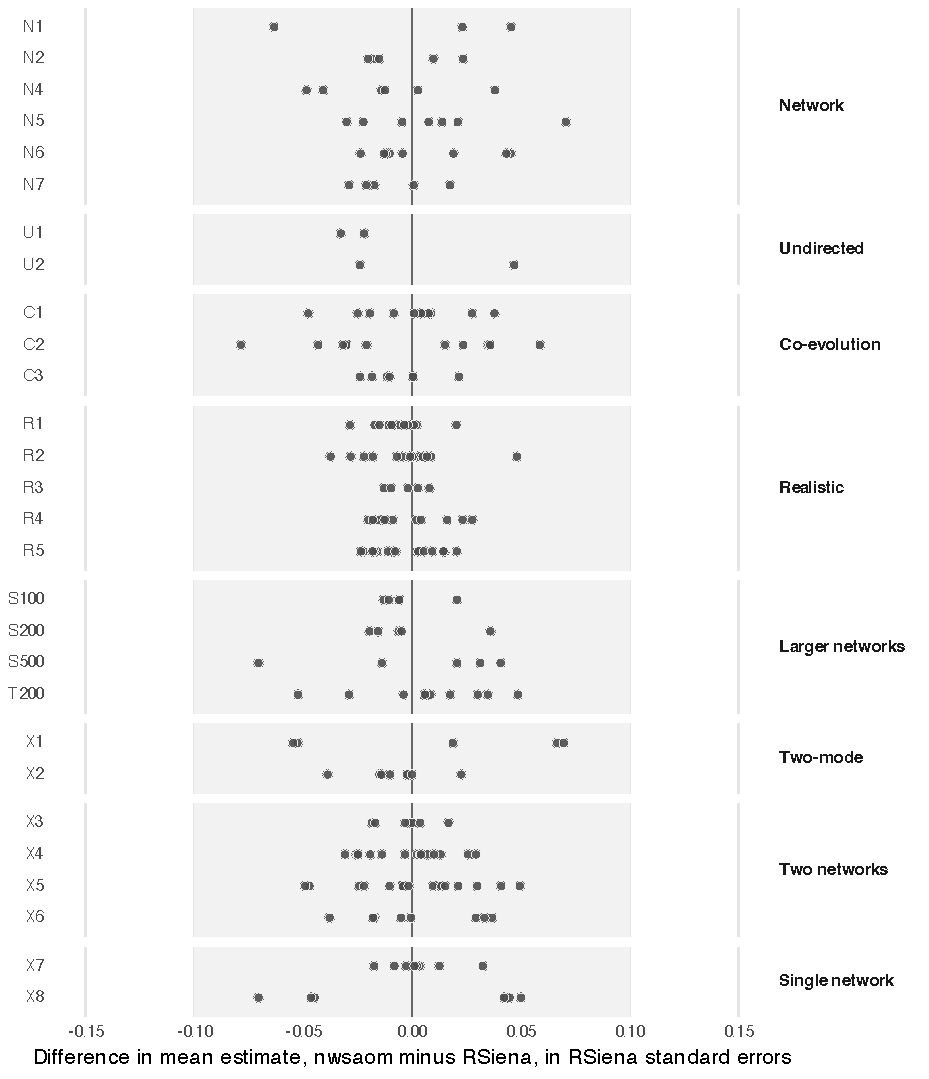
\includegraphics[width=\textwidth]{fig_bench_agree.pdf}
\caption{Difference between the mean estimates of \nwsaom{} and RSiena for every
parameter of every model, in RSiena standard errors; the band marks $\pm0.1$.}
\end{figure}

\section{Further models}\label{sec:benchextra}

The same comparison, with the same conventions (default settings of both programs, a fit counts as converged when RSiena's overall convergence ratio is below 0.25), for the later model families: eight models, X1 and X2 for two-mode networks, X3 to X6 for several networks (with and without a behavior, and with a non-directed network) and X7 and X8 for newer single-network effects. The data are the Glasgow friendship panel, a second randomly generated network and the smoking behavior (several networks), and simulated bipartite data (two-mode).

All eight models agree with RSiena: the largest difference of a mean estimate, rates included, is 0.07 RSiena standard errors.

Some effect sets were chosen so that RSiena converges: on the 40$\times$20 data \texttt{outactivity} together with \texttt{indegpopularity} and \texttt{cycle4} does not converge in RSiena, \texttt{antiiniso2} on the same data and the effects \texttt{Jin} and \texttt{Jout} together on the Glasgow data make \texttt{siena07} stop with ``thetaBound should be set higher'', and the \texttt{Jout} estimate in X8 is large (about 9.6, standard error about 4) in both programs. Some fits did not converge in one of the programs (RSiena: X1 two of eight seeds, X4 and X5 two each, X8 one; \nwsaom{}: X8 one); they are left out of the comparison and replaced by the next seed.

\section{Limits of this comparison}

\begin{itemize}
\item One data set (Glasgow and disconnected copies of it) for the one-mode models, and one specification per family for the later models; agreement may differ for other effects and for sparser or denser networks.
\item Both programs at default settings.
\item RSiena \benchrsiena{} (R \benchrver) was the reference version.
\end{itemize}
